\documentclass[12pt,ngerman]{scrartcl}
\usepackage{tikz}
\usetikzlibrary{positioning}

\begin{document}

\begin{center}
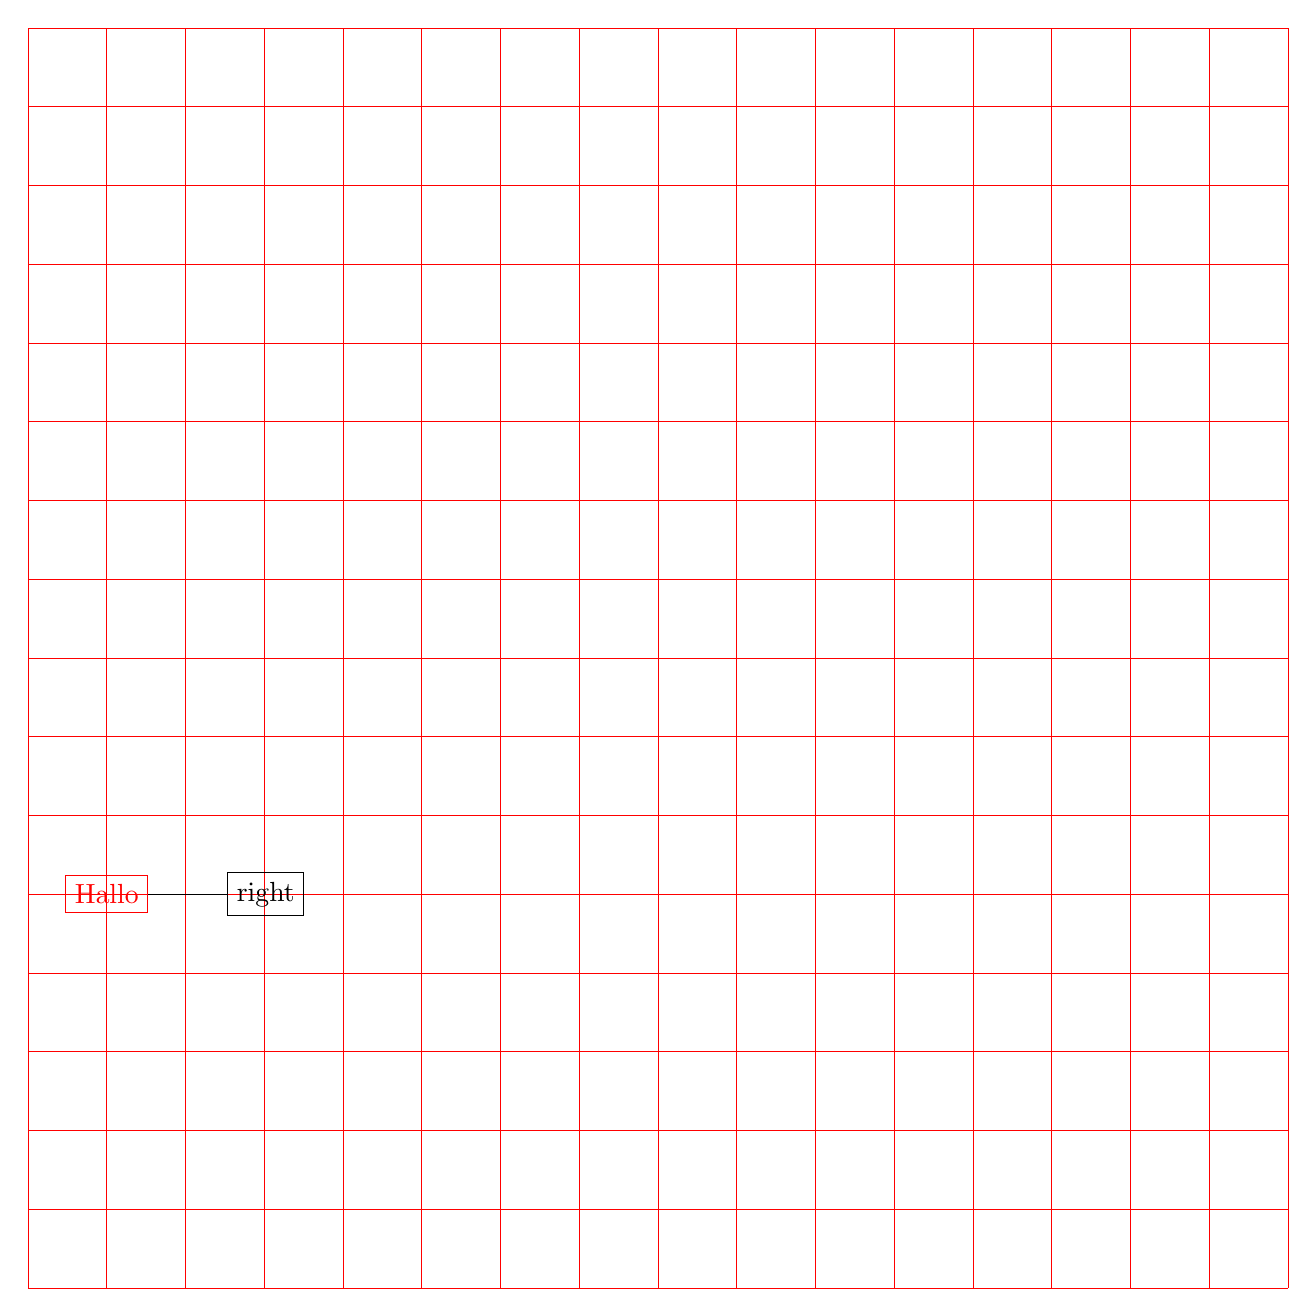
\begin{tikzpicture}
\draw[help lines,red] (0,0) grid (16,16);

\node[rectangle,draw,red](a) at (1,5){Hallo}; 

\node [right =1cm of a,rectangle,draw,black] (b) {right};

\draw(a.east) -- (b);

\end{tikzpicture}
\end{center}


\begin{center}
\resizebox{1cm}{2cm}{%
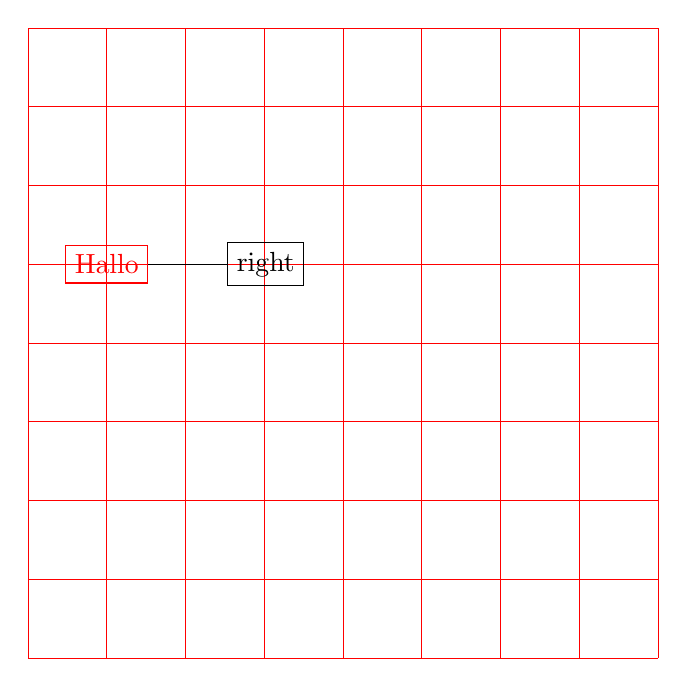
\begin{tikzpicture}
\draw[help lines,red] (0,0) grid (8,8);

\node[rectangle,draw,red](a) at (1,5){Hallo}; 
\node [right =1cm of a,rectangle,draw,black] (b) {right};

\draw(a.east) -- (b);

\end{tikzpicture}
}
\end{center}


\begin{center}
\scalebox{2}{%
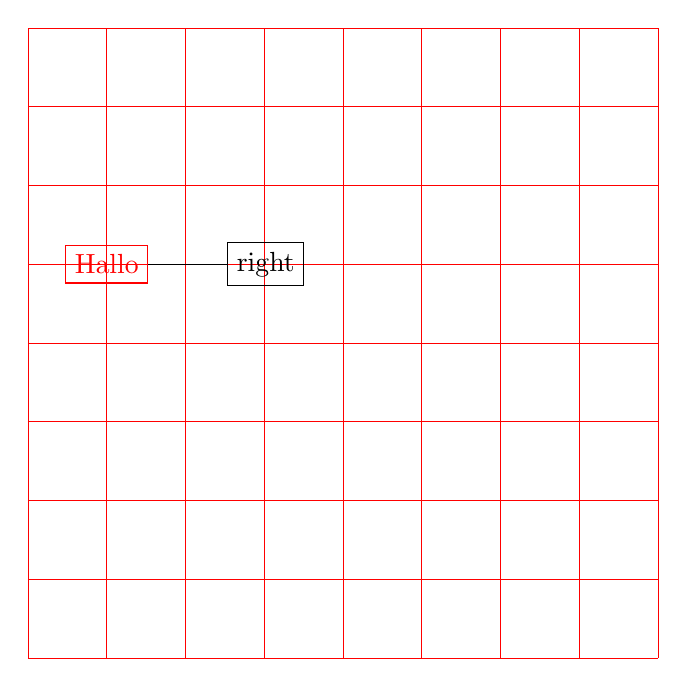
\begin{tikzpicture}
\draw[help lines,red] (0,0) grid (8,8);

\node[rectangle,draw,red](a) at (1,5){Hallo}; 
\node [right =1cm of a,rectangle,draw,black] (b) {right};

\draw(a.east) -- (b);

\end{tikzpicture}
}
\end{center}



\end{document}




\node at (0,0) [box ] (a) {a};
\node [below = of a,box ] (b) {below };
\node [above = of a,box ] (c) {above };
\node [left = of a,box ] (d) {left };
\node [right = of a,box ] (e) {right };
\node [below left = of a,box ] (f) {below left };
\node [below right = of a,box ] (g) {below right };
\node [above left = of a,box ] (h) {above left };
\node [above right = of a,box ] (i) {above right };
